\documentclass[12pt]{article}

\usepackage{amsmath}
\usepackage{multicol}
\usepackage{tikz}
\usetikzlibrary{automata, positioning}

\usepackage[lmargin=2cm, rmargin=5cm]{geometry}
%%%{{{ Comments and the like
\usepackage[textwidth=4cm]{todonotes}
\usepackage{soul}
\usepackage{xcolor}
\newcounter{todocounter}
\newcommand{\comment}[2]{\stepcounter{todocounter}
  {\color{green!50!blue}{(#1$^{{\color{black}\textbf{\thetodocounter}}}$)}}
  \todo[color=green,noline,size=\tiny]{\textbf{\thetodocounter:} #2

  }}
\newcommand{\quitaesto}[1]{{\color{red}(\st{#1})}}

\newcommand{\cambio}[2]{{\color{cyan}{{#2}}}{\color{red}{(\st{#1})}}}

\newcommand{\agregaesto}[1]{{\color{cyan}{{#1}}}}

\newcommand{\notaparaelautor}[1]{{\color{brown}{\textbf{#1}}}}

\newcommand{\errorortografico}[1]{{\fcolorbox{gray}{magenta}{\textcolor{yellow}{\bf #1}}}}
    
%%%}}}

\title{Estrategia para la solución del SAT usando el problema de la palabra}
\author{Raudel Alejandro Gómez Molina}

\begin{document}

\maketitle

En este capitulo se presenta un enfoque distinto al del capítulo anterior, que se basa en definir un lenguaje al cual
pertenecen todos los problemas SAT que son satisfacibles y al cual se le denomina $L_{S-SAT}$, entonces para determinar
si un SAT es satisfacible solo es necesario verificar si pertenece a $L_{S-SAT}$.

\section{Definición de $L_{SAT}$}

El lenguaje de todas las fórmulas booleanas en CNF que son satisfacibles se define como $L_{S-SAT}=\{w\,|\,w \in L_{FULL-SAT} \wedge f_{SAT}(w)\}$, 
donde $L_{FULL-SAT}$ representa el lenguaje de todas las fórmulas booleanas en CNF y $f_{SAT}(w)$ es una función que 
determina si $w$ es satisfacible.

En las próximas secciones se presenta el primer enfoque para definir $L_{S-SAT}$, el cual se basa en definir
el lenguaje mediante un transductor finito seleccionando un formalismo que cumpla ciertas restricciones. 

\section{Transductor SAT}

La idea para definir $L_{S-SAT}$ es construir un transductor finito que acepte como entrada cadenas del lenguaje $L_{0,1}=\{wd\}^+$ donde $w\in \{0,1\}^*$
y tenga como salida cadenas que representan una fórmula booleana en \textit{CNF}  si y solo si la fórmula es satisfacible. 

Detrás de esta construcción se busca asociar cada carácter 0 ó 1 en la cadena de entrada al valor de la variable booleana correspondiente en la cadena de salida y verificar que para dichos
valores al evaluar la fórmula booleana se obtenga un valor de verdad. 

Mediante esta construcción se mantiene la invariante fundamental del SAT que a dos instancias
de la misma variable se les asocia el mismo valor de verdad, esto es posible por como está definido el formato de la cadena de entrada.

A continuación se define el transductor finito $T_{SAT}$ que sigue la construcción definida anteriormente, para ello se define
el transductor $T_{CLAUSE}$ (Figura \ref{fig:transducer}) que hace el proceso de transducción para los valores de verdad de una cláusula $w$, donde $w\in \{0,1\}$:

\[
    T_{CLAUSE} = (Q, {\Sigma}, \Gamma, \delta, q_{0}, F),
\]
donde:
\begin{itemize}
    \item \(Q\) = ${q_0,q_p,q_n}$.
    \item \(\Sigma\) = ${0,1}$.
    \item \(\Gamma\) = ${a,b,c}$.
    \item \(\delta: Q \times \Sigma \to Q \times \Gamma^*\) función de transición.
    \item \(q_{0} = q_0\) estado inicial.
    \item \(F={q_p}\) conjunto de estados finales.
\end{itemize}
se define la función de transición $\delta$ de la siguiente manera:

\begin{itemize}
    \item  transiciones para el estado $q_0$: representa el estado inicial. Si la entrada es un 1 el transductor
          puede escribir $a$, $b$ y $c$ si escriba $a$ pasa al estado positivo, si escribe $b$ pasa al estado negativo
          y si escribe $c$ permanece en el mismo estado. Por otro lado si la entrada es un 0 se intercambian los estados 
          cuando se escribe $a$ y $b$ y cuando se escribe $c$ permanece en el mismo estado.
          
          \begin{multicols}{2}
              \begin{itemize}
                  \item $\delta_{SAT}(q_0,1)=(q_p,a)$
                  \item $\delta_{SAT}(q_0,0)=(q_n,a)$
                  \item $\delta_{SAT}(q_0,1)=(q_n,b)$
                  \item $\delta_{SAT}(q_0,0)=(q_p,b)$
                  \item $\delta_{SAT}(q_0,1)=(q_0,c)$
                  \item $\delta_{SAT}(q_0,0)=(q_0,c)$
              \end{itemize}
          \end{multicols}
          
    \item  transiciones para el estado $q_p$ (estado positivo de $T_{CLAUSE}$): representa que para los valores de verdad de la cláusula obtiene un valor de verdad positivo.
          Como la fórmula se encuentra ya en un estado positivo lo que significa que al menos un literal se evalúa positivo no importa
          la entrada y lo que el transductor escriba se mantiene en el mismo estado.      
          
          \begin{multicols}{2}
              \begin{itemize}
                  \item $\delta_{SAT}(q_{p},1)=(q_{p},a)$
                  \item $\delta_{SAT}(q_{p},0)=(q_{p},a)$
                  \item $\delta_{SAT}(q_{p},1)=(q_{p},b)$
                  \item $\delta_{SAT}(q_{p},0)=(q_{p},b)$
                  \item $\delta_{SAT}(q_{p},1)=(q_{p},c)$
                  \item $\delta_{SAT}(q_{p},0)=(q_{p},c)$
              \end{itemize}
          \end{multicols}
          
    \item  transiciones para el estado $q_n$ (estado negativo de $T_{CLAUSE}$): representa que para los valores de verdad la cláusula obtiene un valor de verdad negativo.
          Aquí las transiciones son idénticas a las del estado inicial, reemplazando el estado inicial por el estado negativo en los posibles resultados
          de la función de transición.       
          
          \begin{multicols}{2}
              \begin{itemize}
                  \item $\delta_{SAT}(q_{n},1)=(q_{p},a)$
                  \item $\delta_{SAT}(q_{n},0)=(q_{n},a)$
                  \item $\delta_{SAT}(q_{n},1)=(q_{n},b)$
                  \item $\delta_{SAT}(q_{n},0)=(q_{p},b)$
                  \item $\delta_{SAT}(q_{n},1)=(q_{n},c)$
                  \item $\delta_{SAT}(q_{n},0)=(q_{n},c)$
              \end{itemize}
          \end{multicols}
\end{itemize}

\begin{figure}[h]
    \centering 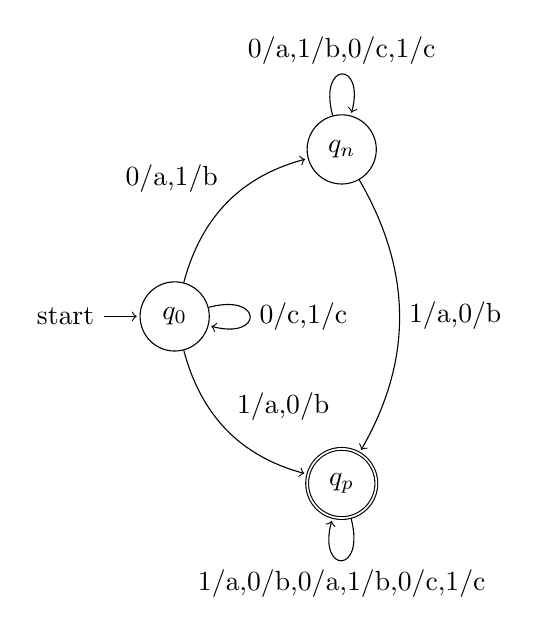
\begin{tikzpicture}[shorten >=1pt, node distance=3cm, on grid, auto]
        
        % Nodos
        \node[state, initial] (q0)   {$q_0$};
        \node[state] (qn) [above right=of q0] {$q_n$};
        \node[state, accepting] (qp) [below right=of q0] {$q_p$};
        
        % Transiciones
        \path[->]
        (q0) edge [bend left] node {0/a,1/b} (qn)
        (q0) edge [bend right] node {1/a,0/b} (qp)
        (q0) edge [loop right] node {0/c,1/c} (q0)
        
        (qn) edge [bend left] node {1/a,0/b} (qp)
        (qn) edge [loop above] node {0/a,1/b,0/c,1/c} (qn)
        
        (qp) edge [loop below] node {1/a,0/b,0/a,1/b,0/c,1/c} (qp);
        
    \end{tikzpicture}
    \caption{Transductor $T_{CLAUSE}$.}
    \label{fig:transducer} % Esto es para referenciar la figura en el texto
\end{figure}

Para definir el transductor $T_{SAT}$ se toman dos instancias del transductor $T_{CLAUSE}$ ($T_1$ y $T_2$ respectivamente) 
y se concatenan añadiendo una transición del estado $q_{p_1}$ (estado positivo de $T_1$) al estado $q_{0_2}$
(estado inicial de $T_2$) con el símbolo $d$ (tanto de lectura como de escritura) y además se agrega una clausura a $T_2$ con una transición del estado $q_{p_2}$ (estado positivo de $T_2$) al estado $q_{0_2}$ con el símbolo $d$ (tanto de lectura como de escritura). Entonces solo resta definir el estado inicial y el estado final de $T_{SAT}$, los cuales serían $q_{0_1}$ (estado inicial de $T_1$) y $q_{0_2}$ (estado inicial de $T_2$), respectivamente.

A continuación se define el lenguaje $L_{S-SAT}$ usando transducción finita.

\subsection{Definición del $L_{S-SAT}$ usando transducción finita}

Finalmente se define $L_{S-SAT}$ como el lenguaje de todas las cadenas $e$ que son aceptadas por el transductor $T_{SAT}$, a partir del lenguaje
de cadenas de entrada $L_{0,1}=\{wd\}^+$ donde $w\in \{0,1\}^*$. 

$$L_{S-SAT} = \{e\,|\,\exists w \in L_{0,1} \wedge e \in T_{SAT}(w) \}$$

Luego $L_{S-SAT}$ contiene todas las fórmulas booleanas satisfacibles, pero este conjunto por si solo no sirve de mucho sin 
un formalismo que permita conocer si una cadena que representa una fórmula booleana pertenece al lenguaje o 
no. Para ello se necesita encontrar un formalismo que sea capaz de generar el lenguaje $L_{0,1}$ y al aplicarle el transductor 
$T_{SAT}$ a dicho formalismo se obtenga un formalismo que cuente con un algoritmo de reconocimiento para reconocer 
si una cadena pertenece a dicho formalismo o no.

Como se evidenció en esta sección encontrar un formalismo que genere el lenguaje $L_{0,1}$, el cual sea cerrado bajo transducción finita
es suficiente para generar el lenguaje $L_{S-SAT}$. Una pregunta interesante sería saber si la existencia de dicho formalismo
es una condición necesaria para definir el lenguaje $L_{S-SAT}$ otra pregunta interesante sería saber si existe un formalismo
que sea capaz de describir el lenguaje $L_{S-SAT}$ y el problema de la palabra en dicho formalismo sea polinomial (observe que de esta manera
se estaría resolviendo el problema \textbf{P vs NP}).

Dado el resultado anterior se puede demostrar que el problema de la palabra de cualquier formalismo que genere el lenguaje 
$L_{0,1}$ y sea cerrado bajo transducción finita es $NP-Duro$, ya que puede ser reducido al SAT y por tanto a cualquier problema
en NP. Para esto habría que demostrar que el lenguaje que genere $L_{S-SAT}$ tiene complejidad O(1).

Ahora se presenta un formalismo que sirve para generar $L_{S-SAT}$ usando el transductor $T_{SAT}$.

\section{$L_{S-SAT}$ como lenguaje de índice global}

En esta sección se presenta una una forma de generar el lenguaje $L_{0,1}$ empleando una GIG. En \cite{globalIndexLanguages} se presenta
una GIG, $G_{ww^+}$ que genera el lenguaje $L(G_{ww^*})=\{ww^+\,|\,w\in\{a,b\}\}$: 
$$
    G_{ww^+} = (N, \Sigma, I, S, \#, P) 
$$
donde:

\begin{itemize}
    \item $N= \{S,R,A,B,C\}$.
    \item \( \Sigma=\{a,b\} \) .
    \item $I=\{i,j\}$.
    \item $S$ es el \textbf{símbolo inicial}.
    \item $\#$ es el \textbf{símbolo inicial de la pila}.
    \item $P$ es un conjunto finito de \textbf{producciones}:
          \begin{multicols}{2}
              \begin{itemize}
                  \item $S\underset{\varepsilon}{\to} AS\,|\,BS\,|\,C$
                  \item $C\underset{\varepsilon}{\to} RC\,|\,L$
                  \item $R\underset{\overline{i}}{\to} RA$
                  \item $R\underset{\overline{j}}{\to} RB$
                  \item $R\underset{[\#]}{\to} \varepsilon$
                  \item $A\underset{i}{\to} a$
                  \item $B\underset{j}{\to} b$
                  \item $L\underset{\overline{i}}{\to} La\,|\,a$
                  \item $L\underset{\overline{j}}{\to} Lb\,|\,b$
              \end{itemize}
          \end{multicols}
\end{itemize}

Observe que la pila en esta gramática es un mecanismo de memoria suficiente para generar \textit{Copy} (el lenguaje \textit{Copy} sobre un alfabeto
$\Sigma$ se define como $L_{copy}=\{ww^+\,|\,w\in Z^*\}$), a cada caracter de $\Sigma$ le corresponde un no terminal y un símbolo de la pila 
por el que se puede producir dicho caracter almacenando el caracter el símbolo de la pila correspondiente, el funcionamiento 
de la gramática lo compone además un mecanismo de recursión por el que se puede producir un no terminal asociado a un caracter
solo eliminando el símbolo de la pila asociado a dicho caracter por último el mecanismo de recursión produce la cadena vacía
solo si el símbolo inicial de la pila se encuentra en el tope.

Entonces dada esta gramática es relativamente realizar una modificación para generar el lenguaje $L_{0,1}$,
a esta nueva gramática se denominará $G_{0,1}$, que se define como:

$$
    G_{0,1} = (N, \Sigma, I, S, \#, P) 
$$
donde:

\begin{itemize}
    \item $N= \{S,R,A,B,C,D\}$.
    \item \( \Sigma=\{0,1,d\} \) .
    \item $I=\{i,j,k\}$.
    \item $S$ es el \textbf{símbolo inicial}.
    \item $\#$ es el \textbf{símbolo inicial de la pila}.
    \item $P$ es un conjunto finito de \textbf{producciones}:
          \begin{multicols}{2}
              \begin{itemize}
                  \item $S\underset{\varepsilon}{\to} AS\,|\,BS\,|\,DC$
                  \item $C\underset{\varepsilon}{\to} RC\,|\,L$
                  \item $R\underset{\overline{i}}{\to} RA$
                  \item $R\underset{\overline{j}}{\to} RB$
                  \item $R\underset{\overline{k}}{\to} RD$
                        
                  \item $R\underset{[\#]}{\to} \varepsilon$
                  \item $A\underset{i}{\to} a$
                  \item $B\underset{j}{\to} b$
                  \item $D\underset{k}{\to} d$
                  \item $L\underset{\overline{i}}{\to} L$
                  \item $L\underset{\overline{j}}{\to} L$
                  \item $L\underset{\overline{k}}{\to} L$
                  \item $L\underset{[\#]}{\to} \varepsilon$
              \end{itemize}
          \end{multicols}
\end{itemize}

Como modificaciones a la gramática anterior se ha introducido un nuevo terminal, 
un no terminal y un símbolo de la pila manteniendo la invariante de correspondencia 
que se mencionó anteriormente entre los elementos de estos 3 conjuntos. Por otro lado se modificaron 
las producciones del no terminal $L$ para que unicamente produzca la cadena vacía eliminando todos los elementos de la pila, 
con ello se puede generar el lenguaje $L_{0,1}$.

Como se mencionó anteriormente las GIG son cerradas bajo transducción finita, por lo que $G_{0,1}$ permite describir
$L_{S-SAT}$ usando el transductor $T_{SAT}$, el único inconveniente para este análisis es que luego de aplicar $T_{SAT}$
a la gramática, se obtiene un gramática ambigua y en estos casos el problema de la palabra para las GIG no es polinomial \cite{globalIndexLanguages}.

\begin{thebibliography}{99}
    
    \bibitem{mainRCGBib}
    Boullier, Pierre.
    \textit{Proposal for a Natural Language Processing Syntactic Backbone}.
    Research Report RR-3342, INRIA, 1998.
    
    \bibitem{propertiesRCGBib}
    Boullier, Pierre.
    \textit{A Cubic Time Extension of Context-Free Grammars}.
    Research Report RR-3611, INRIA, 1999.
    
    \bibitem{simpleMatrixLanguages}
    Ibarra, Oscar H.
    \textit{Simple matrix languages}.
    \textit{Information and Control}, Vol. 17, No. 4, pp. 359-394, 1970.
    
    \bibitem{globalIndexLanguages}
    Castaño, José M.
    \textit{Global Index Languages}.
    Ph.D. Thesis, The Faculty of the Graduate School of Arts and Sciences, Brandeis University, 2004.
    
    \bibitem{authomataTheory}
    Hopcroft, John E., Motwani, Rajeev, y Ullman, Jeffrey D.
    \textit{Introduction to Automata Theory, Languages, and Computation}.
    3ª edición, Addison-Wesley, 2006. ISBN: 9780321455369.
    
    \bibitem{aCFSAT}
    Fernández Arias, Alina.
    \textit{El problema de la satisfacibilidad booleana libre del contexto}.
    Facultad de Matemática y Computación, Universidad de La Habana, 2007.
    
    \bibitem{aSRCSAT}
    Aguilera López, Manuel.
    \textit{Problema de la Satisfacibilidad Booleana de Concatenación de Rango Simple}.
    Facultad de Matemática y Computación, Universidad de La Habana, 2016.
    
    \bibitem{aSMSAT}
    Rodríguez Salgado, José Jorge.
    \textit{Gramáticas Matriciales Simples. Primera aproximación para una solución al problema SAT}.
    Facultad de Matemática y Computación, Universidad de La Habana, 2019.
    
\end{thebibliography}


\end{document}